\documentclass{standalone}

\usepackage[latin1]{inputenc}
\usepackage{amsmath}
\usepackage{amssymb}
\usepackage{amsthm}

\usepackage{tikz}
\usetikzlibrary{arrows,calc}

%% generates a tightly fitting border around the work
%\usepackage[active,tightpage]{preview}
%\PreviewEnvironment{tikzpicture}
%\setlength\PreviewBorder{0.5mm}
%%\renewcommand\PreviewBbAdjust{-\PreviewBorder 1mm -1.15mm -0.85mm}

\usepackage{color}

%\pagestyle{empty}

\begin{document}

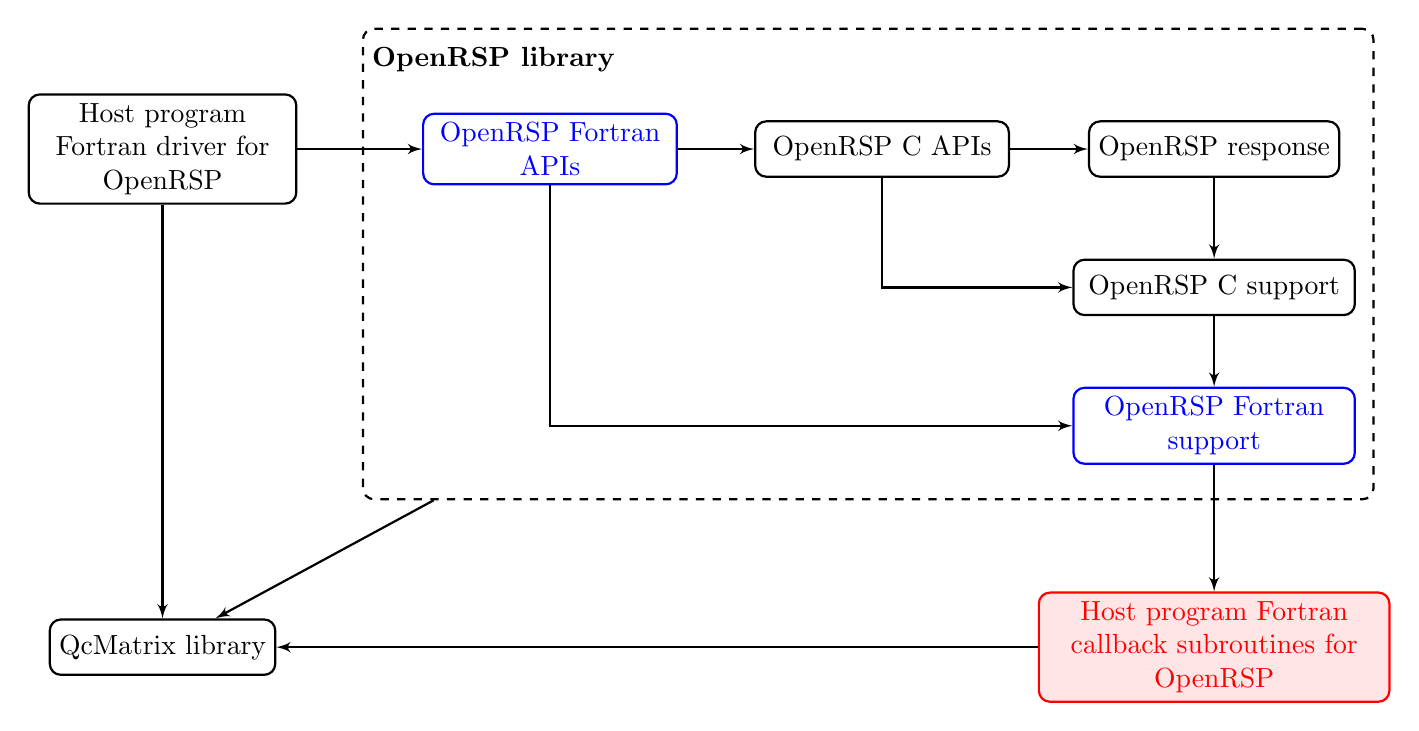
\begin{tikzpicture}[thick]
  \node[color=black, rectangle, draw, text badly centered, rounded corners, %
        minimum height=20] (OpenRSP-response) {OpenRSP response};
  \node[color=black, rectangle, draw, text badly centered, rounded corners, %
        minimum height=20, text width=85, left of=OpenRSP-response, node distance=120] %
       (OpenRSP-C-API) {OpenRSP C APIs};
  \node[color=blue, rectangle, draw, text badly centered, rounded corners, %
        minimum height=20, text width=85, left of=OpenRSP-C-API, node distance=120] %
       (OpenRSP-Fortran-API) {OpenRSP Fortran APIs};
  \node[color=black, rectangle, draw, text badly centered, rounded corners, %
        minimum height=20, text width=95, below of=OpenRSP-response, node distance=50] %
       (OpenRSP-C-support) {OpenRSP C support};
  \node[color=blue, rectangle, draw, text badly centered, rounded corners, %
        minimum height=20, text width=95, below of=OpenRSP-C-support, node distance=50] %
       (OpenRSP-Fortran-support) {OpenRSP Fortran support};
  \node[color=black, dashed, rectangle, draw, text badly centered, rounded corners, %
        minimum height=170, minimum width=280, above of=OpenRSP-C-API, %
        xshift=-5, yshift=-70] (OpenRSP-library) %
       {\begin{minipage}[t][5.5cm]{12.6cm}\textbf{OpenRSP library}\end{minipage}};
%
  \node[color=black, rectangle, draw, text badly centered, rounded corners, %
        minimum height=20, text width=90, left of=OpenRSP-Fortran-API, node distance=140] %
       (HostDriver) {Host program Fortran driver for OpenRSP};
  \node[color=red, fill=red!10, rectangle, draw, text badly centered, rounded corners, %
        minimum height=20, text width=120, below of=OpenRSP-Fortran-support, node distance=80] %
       (Callback) {Host program Fortran callback subroutines for OpenRSP};
%
  \node[color=black, rectangle, draw, text badly centered, rounded corners, %
        minimum height=20, below of=HostDriver, node distance=180] %
       (QcMatrix) {QcMatrix library};
%
  \draw [-latex'] (OpenRSP-Fortran-API)--(OpenRSP-C-API);
  \draw [-latex'] (OpenRSP-C-API)--(OpenRSP-response);
  \draw [-latex'] (OpenRSP-response)--(OpenRSP-C-support);
  \draw [-latex'] (OpenRSP-C-API)|-(OpenRSP-C-support);
  \draw [-latex'] (OpenRSP-C-support)--(OpenRSP-Fortran-support);
  \draw [-latex'] (OpenRSP-Fortran-API)|-(OpenRSP-Fortran-support);
  \draw [-latex'] (OpenRSP-library)--(QcMatrix);
  \draw [-latex'] (HostDriver)--(OpenRSP-Fortran-API);
  \draw [-latex'] (OpenRSP-Fortran-support)--(Callback);
  \draw [-latex'] (HostDriver)--(QcMatrix);
  \draw [-latex'] (Callback)--(QcMatrix);
\end{tikzpicture}

\end{document}
